% Prof. Dr. Ausberto S. Castro Vera
% UENF - CCT - LCMAT - Curso de Ci\^{e}ncia da Computa\c{c}\~{a}o
% Campos, RJ,  2022
% Disciplina: An\'{a}lise e Projeto de Sistemas
% Aluno: 

\chapterimage{planejamento.png} % Table of contents heading image
\chapter{Etapa de Planejamento}


Neste cap\'{\i}tulo \'{e} apresentado os detalhes sobre a implementação
do sistema junto com suas etapas e seu valor agregado.


\section{Solicita\c{c}\~{a}o do Sistema}

\begin{itemize}
       \item Responsavel do sistema: Javier Ernesto Lopez Del Real
       \item Necessidades da empresa
             \begin{itemize}
                    \item Necessidade de praticidade da comunicação de informação entre as agências e análise geral dos dados de forma eficaz
             \end{itemize}
       \item Requisitos do negocio:
             \begin{itemize}
                    \item Integração entre companhias de diferentes aeroportos, controle geral de faturamento de vendas e controle de clientes e aeronaves, junto com a análise de dado realizado com todas essas entidades que fazem parte do sistema
             \end{itemize}
       \item Valor agregado
             \begin{itemize}
                    \item O sistema realiza indiretamente a economia de tempo gasto da equipe, com a análise dos dados será possível controlar melhor as operações identificando processos que precisam ser ajustados gerando inteligência no negócio para tomar melhores decisões.
             \end{itemize}
       \item Outras informações
             \begin{itemize}
                    \item Com a implementação do sistema haverá o aumento
                          numero de passagens vendidas e uma melhor logistica das aeronaves
                          em cada aeroporto.
                          
             \end{itemize}
\end{itemize}


\section{Custos: Desenvolvimento e Operacional}
%%%%%%%%%%%%%%%%%%%%%%%%%%%%%%%
\begin{itemize}
       \item Desenvolvimento
             \begin{itemize}
                    \item Salário da equipe de desenvolvedores
                    \item Custo de hardware e licenças de softwares a serem utilizados
                    \item Treinamento e capacitação de equipe de desenvolvimento e depois dos funcionários
                    \item Custos de escritório
             \end{itemize}
       \item Operacional
             \begin{itemize}
                    \item Salário de equipe operacional
                    \item Custos de instalação e transição para o novo sistema
                    \item Custos de manutenção
                          
             \end{itemize}
\end{itemize}

\section{Benef\'{\i}cios}
%%%%%%%%%%%%%%%%%%%%%%%%%%%%%%%
Dentre os possíveis benefícios deste projeto, estão inclusos benefícios tangíveis e intangíveis
apresentados a seguir:

\subsection{Benef\'{\i}cios Tang\'{\i}veis}
\begin{itemize}
       \item Aumento nas vendas de passagens
       \item Otimização das vendas
       \item Aumento do controle de aeronaves
       \item Facilitação da manutenção das aeronaves
       \item Operacional mais eficaz com analise de dados criada
\end{itemize}



\subsection{Benef\'{\i}cios Intang\'{\i}veis}
\begin{itemize}
       \item Maior satisfação dos clientes
       \item Aumento da produtividade dos funcionarios
       \item Maior custo beneficio das aeronaves
\end{itemize}


\section{Estudo de Viabilidade}
%%%%%%%%%%%%%%%%%%%%%%%%%%%%%%%
Nesta seção serão examinados aspectos que influenciam a viabilidade do projeto, levando a uma
conclusão.

\subsection{Calend\'{a}rio }
\begin{itemize}
       \item Inicio do projeto: 07/03/2022
       \item Planejamento do sistema: de 07/03/2022 à 07/05/2022
       \item Análise do sistema: de 07/05/2022 à 07/07/2022
       \item Projeto do sistema: de 07/07/2022 à 07/09/2022
       \item Implementação do sistema: de 07/09/2022 à 07/03/2023
       \item Fim do projeto: 07/03/2023
\end{itemize}


\subsection{Cronograma}
\begin{figure}[h]
 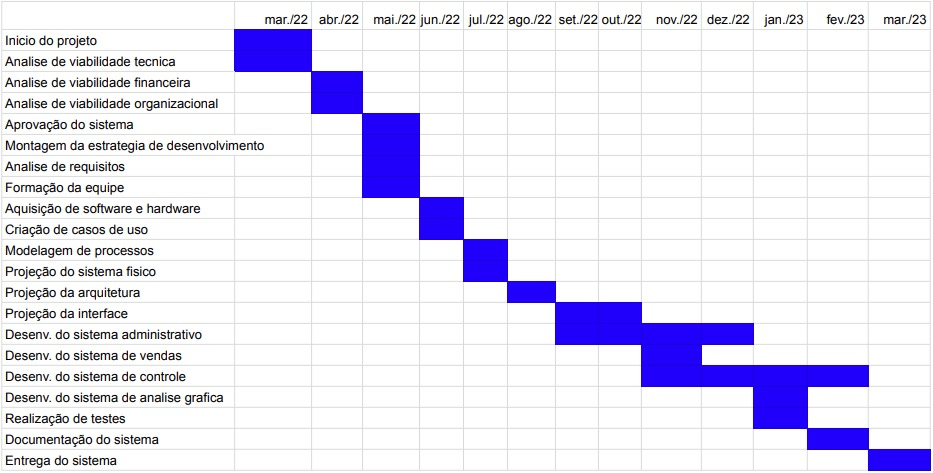
\includegraphics[width=15cm]{cronograma.png}
\end{figure}



\subsection{Or\c{c}amento }

\begin{tabular}{lllll}
       Quantidade & Componentes       & Preço/Unidade(R) & Valor Total &  \\
                  & \textbf{hardware} &                    &             &  \\
                  &                   &                    &             &  \\
       10         & Monitores         & 300,00             &             & 
\end{tabular}



\subsection{Recomenda\c{c}\~{o}es}
Recomenda-se que além da aquisição dos componentes
apresentados na tabela de orçamento, seja
feita a manutenção das necessidades que
forem surgindo no decorrer do projeto para adaptação as
mudanças.

\subsection{Conclus\~{a}o de Viabilidade}
Após o estudo de viabilidade, levando em consideração
que o orçamento do sistema e seu crono-
grama de desenvolvimento se encaixa nas
necessidades e limitações do cliente, conclui-se que o
sistema de integracao e Otimização de processos é 
viavel.

